\chapter{Ergebnisse}
Die verwendete Fe(100)-Oberfläche wurde gefertigt, 
indem ein dünner Eisenfilm (ca. $200\,\si{\nano\meter}$\,-\,$400\,\si{\nano\meter}$) auf einen MgO(100)-Kristall aufgedampft wurde.

Um eine saubere Fe(100)-Oberfläche zu erhalten,
wurde die Probe zunächst durch mehrere Sputter- und Heizdurchgänge
gereinigt. Bei je einem Durchgang wurde bei einer Spannung von $U=1\,\si{\kilo\volt}$ und 
einem Argondruck von $p=1\cdot 10^{-5}\,\si{\milli\bar}$ für 
$15\,\si{\minute}$ gesputtert
und für $5\,\si{\minute}$ bei einer Temperatur von $T=600\,\si{\celsius}$ geheizt. Mittels Auger-Spektren und LEED-Bildern 
wurde die Reinheit und Ordnung der Oberfläche überprüft. 
Solch ein Auger-Spektrum und ein LEED-Bild von der sauberen Fe(100) Oberfläche sind in den Abbildungen \ref{fig:Auger1} 
(oben) und  \ref{fig:LEED} (a) zu sehen.



Auf der gereinigten Probe wurde nun das MgO-Wachstum einzelner Monolagen untersucht.
Die Mg-Aufdampfrate wurde mittels der QCM bestimmt 
und damit anschließend bei passendem Sauerstoffdruck nach Zusammenhang \ref{eq:V1} 
eine MEED-Messung des Wachstums von MgO bei einer Probentemperatur von $T=170\,\si{\celsius}$
für $22\,\si{\minute}$ auf dem sauberen Eisen durchgeführt. 
Eine höhere Temperatur erleichtert zwar das lagenweise Wachstum, doch 
nach Tekiel et al. sinkt die kristalline Ordnung bei Temperaturen über $T=160\,\si{\celsius}$ \cite{tekiel2013reactive}. 
Wegen der Distanz des Thermoelements zur Probe wurde hier eine etwas höhere Temperatur von $T=170\,\si{\celsius}$ gewählt.

Um den Prozess mit Auger-Spektren, LEED-Bildern und IV-Kurven zu untersuchen, wurde das gleiche Wachstum noch einmal 
sukzessive durchgeführt. Dabei wurde die Probe je einmal vollständig mit diesen Methoden vermessen und anschließend 
bei den gleichen Einstellungen wie oben Magnesium nacheinander für je $t=116\,\si{\second}$, $t=250\,\si{\second}$, $t=597\,\si{\second}$ 
und $t=251\,\si{\second}$ in Sauerstoffatmosphäre aufgedampft.

Für den Vergleich mit dem Wachstum von MgO auf passivertem Eisen wurde auch dieses System vermessen.
Zur Passiverung wurde die saubere Eisenprobe zunächst für $5\,\si{\minute}$ bei einer Temperatur von $T=550\,\si{\celsius}$ 
und einer Sauerstoffatmosphäre mit 
$p=1,3\cdot 10^{-7}\,\si{\milli\bar}$ ausgesetzt, was $30\,\symup{L}$ entspricht. 
Nach \cite{picone2016controlling} bildet sich auf diese Weise eine Fe(100)-p(1\,x\,1)O Struktur.
\newpage
\section{Schichtdicken-Charakterisierung mittels MEED und AES}

In Abbildung \ref{fig:QCM1} ist die aufgedampfte Mg-Schichtdicke in Abhängigkeit der Zeit aufgetragen.
Im Bereich von $t=400\,\si{\second}$ bis $t=600\,\si{\second}$ wurde der Aufdampfer mit einem Flux von $130\,\si{\nano\ampere}$ betrieben, 
welcher als finale Einstellung auch beim MgO-Wachstum verwendet wurde.

\begin{SCfigure}
  \centering
  \includegraphics[scale=1, width=0.5\linewidth]{Plots/QCM_Layout.pdf}
  \caption{Aufgedampfte Mg-Schichtdicke auf der QCM vor und nach dem Öffnen des Shutters.
          Aus der Änderung der Schichtdicke mit der Zeit ergibt sich eine Aufdampfrate von $r=0,34\,\si{\angstrom\per\minute}$.}
  \label{fig:QCM1}
\end{SCfigure}

Aus der dadurch resultierenden Aufdampfrate von $r=0,34\,\si{\angstrom\per\minute}$ und dem verwendeten 
Sauerstoffdruck $p=3\cdot 10^{-8}\,\si{\milli\bar}$ ergibt sich ein Verhältnis von

\begin{equation*}
  \frac{r}{p}=0,11\cdot 10^8 \,\si{\angstrom\per\milli\bar\per\minute},
\end{equation*}

welches im Bereich $r/p=(0,15\pm 0,05)\cdot 10^8 \,\si{\angstrom\per\milli\bar\per\minute}$ (siehe Abschnitt \ref{sec:Wachstum}) liegt.

\begin{figure}[H]
  \centering
  \includegraphics[scale=1, width=0.7\linewidth]{Plots/MEED-Original-2_Layout.pdf}
  \caption{MEED-Spektrum des MgO-Wachstums auf Fe(100). Aufgedampft wurde mit einer Rate von $r=0,34\,\si{\angstrom\per\minute}$ 
          bei einem Sauerstoffdruck von $p=3\cdot 10^{-8}\,\si{\milli\bar}$.}
  \label{fig:MEED1}
\end{figure}

Der in Abbildung \ref{fig:MEED1} gezeigte MEED-Verlauf zeigt die Maxima der ersten zwei vollen Monolagen nach $106\,\si{\second}$ und weiteren $281\,\si{\second}$.
Aufgrund des starken Untergrunds lässt sich das Maxima der dritten Monolage nicht so eindeutig und  das der vierten Monolage gar nicht zuordnen, 
doch der relative Verlauf und die Ergebnisse der späteren Auswertung der Augerpeak Verhältnisse lässt darauf schließen, dass sich
die dritte Monolage nach weiteren $352\,\si{\second}$ und die vierte Monolage sich nach weiteren $345\,\si{\second}$ bildet. 

Auffällig ist hier, dass die Wachstumszeit für eine volle Monolage nicht konstant ist, sondern sich einem Grenzwert von ca. $350\,\si{\second}$ annähert.

Aus der Mg-Aufdampfrate der QCM lässt sich eine Vorhersage für die MgO-Wachstumsrate erstellen. Dazu wird angenommen, dass 
bei einem MgO-Kristall die Hälfte der Gitterplätze mit Sauerstoffatomen belegt ist, wodurch sich die MgO-Wachstumsrate gegenüber der Mg-Aufdampfrate
verdoppeln würde. Jedoch ist auch die Dichte von MgO um den Faktor $\rho_{\symup{MgO}}/\rho_{\symup{Mg}}=2,06$ größer als die von Mg, weshalb
sich die Wachstumsrate durch die dichtere Anordnung verringert. Insgesamt ergibt sich so $r_{\symup{Wachstum,\, QCM}}=0,97\cdot r=0,33\,\si{\angstrom\per\minute}$.
Zwischen der so ermittelten und der gemessenen Wachstumsrate $r_{\symup{Wachstum,\, MEED}}=0,36\,\si{\angstrom\per\minute}$ von MgO (angenommen wurde eine Schichtdicke von 2,105$\si{\angstrom}$) 
besteht also ein Faktor 

\begin{equation*}
  \frac{r_{\symup{Wachstum,\, MEED}}}{r_{\symup{Wachstum,\, QCM}}}=1,09.
\end{equation*}

Um die variierende Wachstumszeit genauer zu untersuchen, wird eine 
weitere MEED-Messung des Wachstums von MgO auf Fe(100) und Fe(100)-p(1\,x\,1)O 
zum Vergleich der beiden Systeme betrachtet.
Die Aufdampfrate für diese Messung wurde 
mittels der QCM zu $r=0,45\,\si{\angstrom\per\minute}$ bestimmt (Abbildung \ref{fig:QCM2}).

\begin{SCfigure}
  \centering
  \includegraphics[scale=1, width=0.5\linewidth]{Plots/QCM_2021_07_21_Layout.pdf}
  \caption{Aufgedampfte Mg-Schichtdicke auf der QCM vor und nach dem Öffnen des Shutters.
  Aus der Änderung der Schichtdicke mit der Zeit ergibt sich eine Aufdampfrate von $r=0,45\,\si{\angstrom\per\minute}$.}
  \label{fig:QCM2}
\end{SCfigure}



\begin{figure}[H]
  \centering
  \includegraphics[scale=1, width=0.7\linewidth]{Plots/MEED_2021_07_21_FeO_u_Fe_Layout.pdf}
  \caption{MEED-Messungen des MgO-Wachstums auf Fe(100) (orange) und Fe(100)-p(1\,x\,1)O (blau). Die Messungen wurden um einen linear verlaufenden Untergrund korrigiert.
          Aufgedampft wurde mit einer Rate von $r=0,45\,\si{\angstrom\per\minute}$ 
          bei einem Sauerstoffdruck von $p=4\cdot 10^{-8}\,\si{\milli\bar}$.}
  \label{fig:MEED2}
\end{figure}

Die Oszillationen im MEED-Verlauf \ref{fig:MEED2} sind bei dieser Messung deutlich zu erkennen und können durchgängig 
den vollen Monolagen des Wachstums zugeordnet werden. Beim passivierten Eisen ist die Wachstumszeit nahezu konstant bei $258\,\si{\second}$ für eine volle Monolage.
Auch hier stellt sich der Faktor von

%Die Oszillationen im MEED Verlauf \ref{fig:MEED2} sind bei dieser Messung deutlich zu erkennen und können durchgängig eindeutig 
%den vollen Monolagen des Wachstums zugeordnet werden. Hierbei ist die Wachstumszeit nahezu konstant bei $258\,\si{\second}$ für eine volle Monolage.
%Auch hier stellt sich der Faktor von
%
\begin{equation*}
  \frac{r_{\symup{Wachstum,\, MEED}}}{r_{\symup{Wachstum,\, QCM}}}=1,09
\end{equation*} 

zwischen der Wachstumsrate $r_{\symup{Wachstum,\, QCM}}=0,97\cdot r=0,44\,\si{\angstrom\per\minute}$ und 
der bestimmten Wachstumsrate $r_{\symup{Wachstum,\, MEED}}=0,48\,\si{\angstrom\per\minute}$ ein.

Es ist wieder zu beobachten, dass die ersten zwei ML auf dem reinen Eisen schneller wachsen als die Nachfolgenden.
Später stellt sich die gleiche Wachstumszeit für eine ML ein wie beim passivierten Eisen.
Dies lässt sich auf die hohe Reaktivität der reinen Eisenoberfläche zurückführen.
Während also bei dem MgO Wachstum auf reinem Eisen der Sauerstoff besonders schnell auf der Eisenoberfläche adsorbiert, 
so ist das passivierte Eisen schon mit Sauerstoff gesättigt und das Wachstum von Beginn an gleichbleibend schnell.

Die Schichtdickenbestimmung mit AES-Spektren wurde bei MgO-Wachstum auf sauberem Fe(100) durchgeführt.
Die aufgenommenen Spektren des sukzessiven Wachstums sind in Abbildung \ref{fig:Auger1} dargestellt.

\begin{SCfigure}
  \centering
  \includegraphics[scale=1, width=0.7\linewidth]{Plots/Auger_Vergleich_Layout.pdf}
  \caption{Auger-Spektren im Energiebereich $E=200-1250\, \si{\eV}$ nach unterschiedlicher Aufdampfdauer. 
          Die Bestimmung der Anzahl der ML erfolgt später durch \ref{fig:Auger-Verhältnisse2}. Durch einen Savitzky-Golay Filter 2.\nobreakspace Ordnung mit 9 Punkten wurden die
          Auger-Spektren geglättet.}
  \label{fig:Auger1}
\end{SCfigure}



\begin{figure}[H]
  \centering
  \includegraphics[width=\linewidth]{Plots/Auger-Verhältnisse-Schichtdicke_2_Layout.pdf}
  \caption{Augerpeak-Verhältnisse in Abhängigkeit der Schichtdicke errechnet mit Gleichung \ref{eq:Auger-V}, für die verschiedenen
           mittleren freien Weglängen aus \ref{tab:AugerS}. Dabei geben die blauen Kurven das O/Fe Verhältnis und die schwarzen Kurven das Mg/Fe Verhältnis an.
           Die Kreuze kennzeichnen die gemessenen Verhältnisse nach ausgewählten Aufdampfdauern.}
  \label{fig:Auger-Verhältnisse1}
\end{figure}

Die Auswertung der Verhältnisse der Peaks für verschiedene mittlere freie Weglängen nach Gleichung \ref{eq:Auger-V} ist in Abbildung \ref{fig:Auger-Verhältnisse1} zu sehen.
Dabei stimmen die Schichtdicken der Mg/Fe und der O/Fe-Verhältnisse mit den mittleren freien Weglängen von Seah et al. \cite{seah1979quantitative} am besten überein.
Diese sind noch einmal in Abbildung \ref{fig:Auger-Verhältnisse2} dargestellt.

\begin{SCfigure}
  \centering
  \includegraphics[width=0.7\linewidth]{Plots/Auger-Verhältnisse-Schichtdicke_Layout.pdf}
  \caption{Augerpeak-Verhältnisse in Abhängigkeit der Schichtdicke errechnet mit Gleichung \ref{eq:Auger-V} und den mittleren freien Weglängen von Seah et al. \cite{seah1979quantitative}, je einmal für das Mg/Fe- und das O/Fe-Verhältnis.
          Die Kreuze kennzeichnen die gemessenen Verhältnisse nach ausgewählten Aufdampfdauern.}
  \label{fig:Auger-Verhältnisse2}
\end{SCfigure}


Auf diese Weise lassen sich den Wachstumszeiten jeweils präzise MgO-Schichtdicken zuordnen.
Da es sich um unterschiedliche Wachstumsdurchläufe handelt,
lassen sich die Ergebnisse nur bedingt auf die MEED-Messung \ref{fig:MEED1} übertragen, 
weichen jedoch auch dort nur um maximal $0,5$\,ML von der bestimmten Schichtdicke ab.


\section{Elementanalyse mittels AES}


Aus den aufgenommenen Auger-Spektren \ref{fig:Auger1} lässt sich durch Gleichung \ref{eq:AugerK} die Konzentration der Elemente an der Oberfläche bestimmen,
siehe Tabelle \ref{tab:AugerT}.


\begin{table}
  \centering
  \begin{tabular}{S| S S S S S}
    \toprule
    {$\symup{Element}$} & {$0\,\symup{ML}$} & {$1\,\symup{ML}$} & {$1,6\,\symup{ML}$} & {$3,5\,\symup{ML}$} & {$4,3\,\symup{ML}$}\\
    \midrule
    $\symup{Fe}$ & {$100\,\si{\percent}$} & {$77\,\si{\percent}$} & {$66\,\si{\percent}$} & {$44\,\si{\percent}$} & {$37\,\si{\percent}$}\\
    $\symup{O}$ & {$0\,\si{\percent}$} & {$11\,\si{\percent}$} & {$20\,\si{\percent}$} & {$32\,\si{\percent}$} & {$36\,\si{\percent}$}\\
    $\symup{Mg}$ & {$0\,\si{\percent}$}& {$12\,\si{\percent}$}& {$14\,\si{\percent}$}& {$24\,\si{\percent}$}& {$27\,\si{\percent}$}\\
    \bottomrule
  \end{tabular}
  \caption{Konzentration der vorhandenen Elemente an der Oberfläche nach sukzessivem Wachstum von MgO auf Fe(100).}
  \label{tab:AugerT}
\end{table}

Während zu Beginn die Konzentration des Magnesiums noch gleich der von Sauerstoff ist, stellt sich nach dem zweiten Wachstum ein 
Sauerstoffüberschuss ein. Es scheint also sinnvoll, den Sauerstoffdruck nach der ersten Monolage zu senken, was den Ergebnissen aus \cite{tekiel2013reactive} widerspricht.
Tekiel et al. fanden ein besseres Mg/O-Verhältnis bei niedrigeren Sauerstoffdrücken zu Beginn des Wachstums während der 
ersten Monolage, mit darauf folgenden höheren Sauerstoffdrücken.

Es ist jedoch wichtig anzumerken, dass der Mg-Peak durch die geringe Sensitivität $S=0,1$ bei sehr geringer Konzentration an
der Oberfläche nur schwer vom Untergundrauschen der Augerspektren zu unterscheiden ist. 

\begin{SCfigure}
  \centering
  \includegraphics[scale=1, width=0.69\linewidth]{Plots/Auger_Vergleich__FeO_Layout.pdf}
  \caption{Auger-Spektren im Energiebereich $E=200-1200\, \si{\eV}$ bei unterschiedlichen Schichtdicken von MgO auf Fe-p(1\,x\,1)O. 
          Durch einen Savitzky-Golay Filter 2. Ordnung mit 9 Punkten wurden die
          Auger-Spektren geglättet.}
  \label{fig:Auger2}
\end{SCfigure}



\begin{table}[H]
  \centering
  \begin{tabular}{S| S S S}
    \toprule
    {$\symup{Element}$} & {$0\,\symup{ML}$} & {$1,1\,\symup{ML}$} & {$2,5\,\symup{ML}$}\\
    \midrule
    $\symup{Fe}$ & {$89\,\si{\percent}$} & {$71\,\si{\percent}$} & {$61\,\si{\percent}$}\\
    $\symup{O}$ & {$11\,\si{\percent}$} & {$19\,\si{\percent}$} & {$21\,\si{\percent}$}\\
    $\symup{Mg}$ & {$0\,\si{\percent}$}& {$10\,\si{\percent}$}& {$18\,\si{\percent}$}\\
    \bottomrule
  \end{tabular}
  \caption{Konzentration der vorhandenen Elemente an der Oberfläche nach sukzessivem Wachstum von MgO auf Fe(100)-p(1\,x\,1)O.}
  \label{tab:AugerT2}
\end{table}

Für MgO auf dem passivierten Eisen sind die Auger-Spektren in Abbildung \ref{fig:Auger2} dargestellt und die errechneten Konzentrationen 
in Tabelle \ref{tab:AugerT2} aufgeführt. Während die Mg-Konzentration vergleichbar ist mit der des Wachstum auf reinem Fe(100),
bleibt die Sauerstoffkonzentration beim passivierten Eisen auch nach dem Wachstum weniger Monolagen erhöht. 
Dies zeigt widerum, dass die reine Eisenprobe nicht
sofort passiviert wird, wenn für das Wachstum eine Sauerstoffatmopshäre in der Größenordnung $p=3\cdot 10^{-8}\,\si{\milli\bar}$ eingestellt wird. 
Weiterführend dazu fanden Cattoni et al. \cite{PhysRevB.80.104437} mittels Röntgenphotoelektronenspektroskopie-Messungen heraus, dass keine Fe-O Interaktionen an der Fe(100)/MgO-Grenzfläche 
stattfinden. Die physikalischen Eigenschaften der reinen Eisenoberfläche bleiben im Falle eines 
Fe(100)/MgO-Systems im Vergleich zu einem Fe(100)-p(1\,x\,1)O/MgO-System also erhalten. Zudem wurde bei diesen Schichtsystemen 
eine erhöhte Austauschaufspaltung für die nicht-passivierte Oberfläche beobachtet.


\section{LEED- und IV-LEED-Messungen}


\begin{figure}[H]
  \centering
  \subfloat[][]{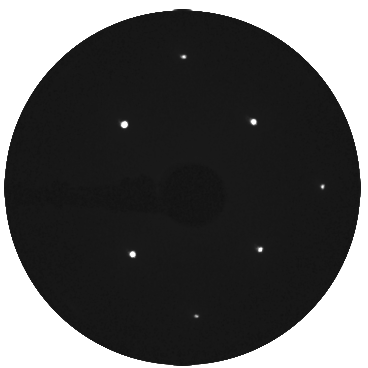
\includegraphics[width=0.25\linewidth]{Plots/LEED_neu/clean_Fe.png}}%
  \qquad
  \subfloat[][]{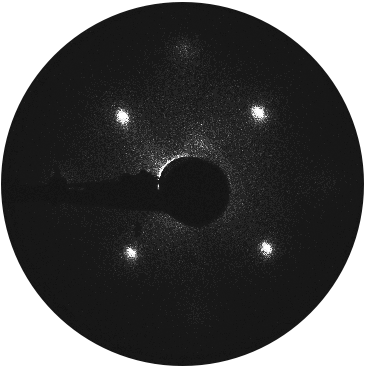
\includegraphics[width=0.25\linewidth]{Plots/LEED_neu/1ML_Fe.png}}%
  \qquad
  \subfloat[][]{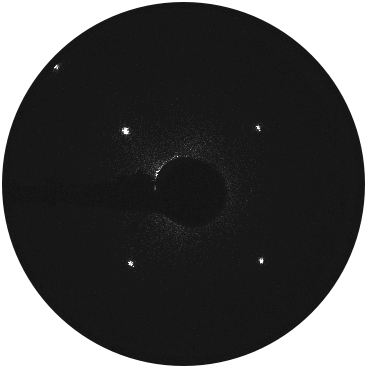
\includegraphics[width=0.25\linewidth]{Plots/LEED_neu/1_6ML_Fe.png}}%
  \qquad
  \subfloat[][]{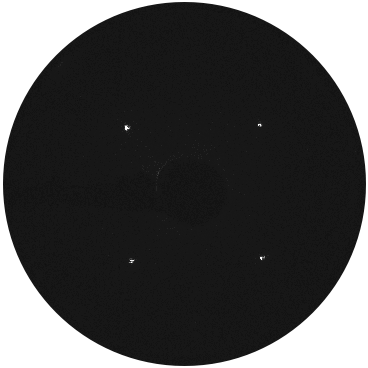
\includegraphics[width=0.25\linewidth]{Plots/LEED_neu/2ML_Fe.png}}%
  \qquad
  \subfloat[][]{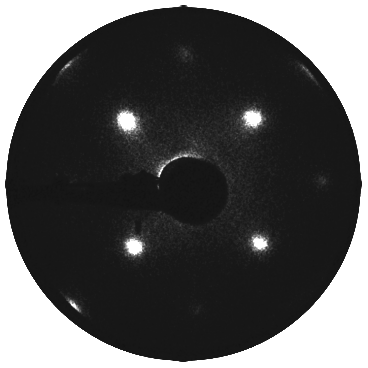
\includegraphics[width=0.25\linewidth]{Plots/LEED_neu/3_5ML_Fe.png}}%
  \qquad
  \subfloat[][]{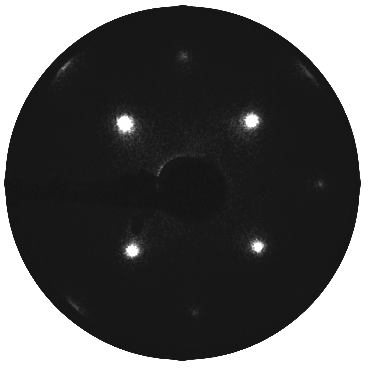
\includegraphics[width=0.25\linewidth]{Plots/LEED_neu/4_3ML_Fe.png}}%
  \caption{LEED-Bilder nach unterschiedlichen Aufdampfdauern von MgO auf Fe(100) bei einer Energie von $E=96\,\si{\eV}$. (a) zeigt sauberes Fe(100),
          (b) eine $1$\,ML Schicht, (c) eine $1,6$\,ML Schicht, (d) eine $2$\,ML Schicht, (e) eine $3,5$\,ML Schicht und (f) eine $4,3$\,ML Schicht.}%
  \label{fig:LEED}
\end{figure}


In Abbildung \ref{fig:LEED} sind auf den LEED-Bildern bei den gleichen Energien $E=96\,\si{\eV}$
die Reflexe bei verschiedenen Schichtdicken von MgO auf reinem Fe(100) zu sehen. 
Die LEED-Bilder können genutzt werden, um eine starke oder schwächere Ordnung der Oberfläche zu 
erkennen und so zum Beispiel zu beurteilen, ob das Wachstum auf der gesamten Probe gleichmäßig verlaufen ist.  
Die unterschiedliche Schärfe der Reflexe ist hier wahrscheinlich auf die unterschiedlichen zugrundeliegenden Wachstumsbedingungen zurückzuführen.



Bei den LEED-Bildern von MgO auf Fe(100)-p(1\,x\,1)O \ref{fig:LEED1}, welche alle im gleichen Wachstumsprozess bei ähnlichen Einstellungen aufgenommen wurden,
ist eine nachlassende Schärfe der Reflexe bei teilweise gefüllten Monolagen zu sehen. 
Bei einer Schichtdicke von $1,1$\,ML liegt eine fast gefüllte ML vor, sodass die Schärfe im Vergleich zur sauberen
Probe etwas nachlässt. Die Reflexe der $2,5$\,ML Schicht sind noch diffuser, 
was sich durch die halbzahlige ML und die dadurch entstehende geringe Ordnung erklären lässt.


%Bei einer Schichtdicke von $1,1$\,ML liegt eine fast gefüllte ML vor,
%die Schärfe lässt im Vergleich zur sauberen Probe etwas nach, 
%bei $2,5$\,ML lässt sie weiter nach, was sich durch die halbzahlige ML und die dadurch entstehende geringe Ordnung erklären lässt.


\begin{figure}[H]
  \centering
  \subfloat[][]{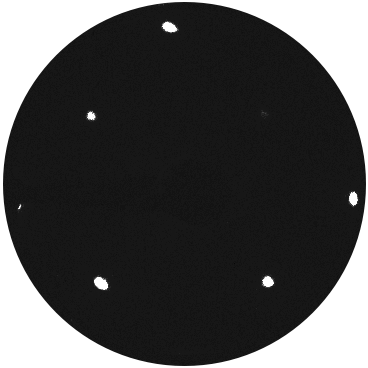
\includegraphics[width=0.25\linewidth]{Plots/LEED_neu/clean_FeO.png}}%
  \qquad
  \subfloat[][]{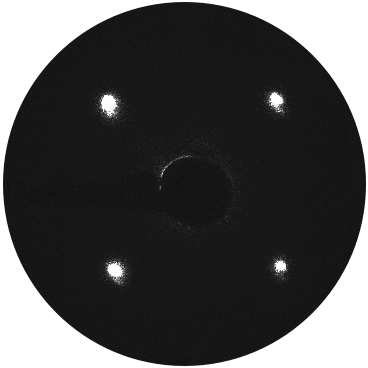
\includegraphics[width=0.25\linewidth]{Plots/LEED_neu/1_1ML_FeO.png}}%
  \qquad
  \subfloat[][]{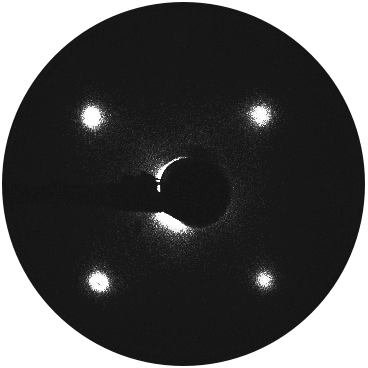
\includegraphics[width=0.25\linewidth]{Plots/LEED_neu/2_5ML_FeO.png}}%

  \caption{LEED-Bilder nach unterschiedlichen Aufdampfdauern von MgO auf Fe(100)-p(1\,x\,1)O bei einer Energie von $E=65\,\si{\eV}$. (a) zeigt die saubere Fe(100)-p(1\,x\,1)O Probe,
          (b) eine $1,1$\,ML Schicht und (c) eine $2,5$\,ML Schicht.}%
  \label{fig:LEED1}
\end{figure}

In Abbildung \ref{fig:LEED2} sind zwei LEED-Bilder von $1,6$\,ML MgO auf reinem Fe(100) zu sehen.
Dabei wurde \ref{fig:LEED2}(a) vor einem schnellen Aufheizen auf $T=600\,\si{\celsius}$ aufgenommen und \ref{fig:LEED2}(b)
danach. Die klareren Reflexe nach dem Aufheizen sprechen für eine bessere Ordnung des Systems.
Dies könnte auf das Entstehen größerer MgO-Domänen hindeuten oder auf das stellenweise Wachstum von Inseln, 
welche durch das Aufheizen aufgebrochen werden.
%was 
%darauf hindeutet, dass Inselstrukturen aufgelöst wurden \ref{sec:Wachstum}. Die  unvollständige Ordnung durch die unbeendete Monolage konnte also 
%durch das Heizen doch noch verbessert werden.

\begin{figure}[H]
  \centering
  \subfloat[][]{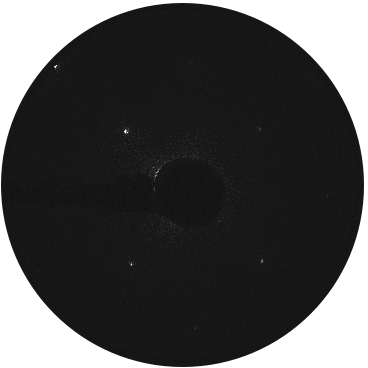
\includegraphics[width=0.25\linewidth]{Plots/LEED_neu/1_6_ML_Fe_96eV_vor_annealen.png}}%
  \qquad
  \subfloat[][]{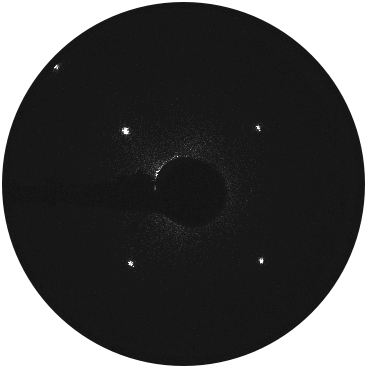
\includegraphics[width=0.25\linewidth]{Plots/LEED_neu/1_6_ML_Fe_96eV_nach_annealen.png}}%
  \caption{LEED-Bilder einer $1,6$\,ML Schicht MgO auf Fe(100) bei einer Energie von $E=96\,\si{\eV}$. (a) zeigt die Probe vor dem Aufheizen,
          (b) zeigt die Probe nach dem Aufheizen.}%
  \label{fig:LEED2}
\end{figure}




\begin{figure}[H]
  \centering
  \begin{subfigure}{0.47\textwidth}
    \includegraphics[width=\textwidth]{Plots/IV-clean_Layout.pdf}
    \caption{}
  \end{subfigure}
  \begin{subfigure}{0.47\textwidth}
    \vspace{-0.2cm}
    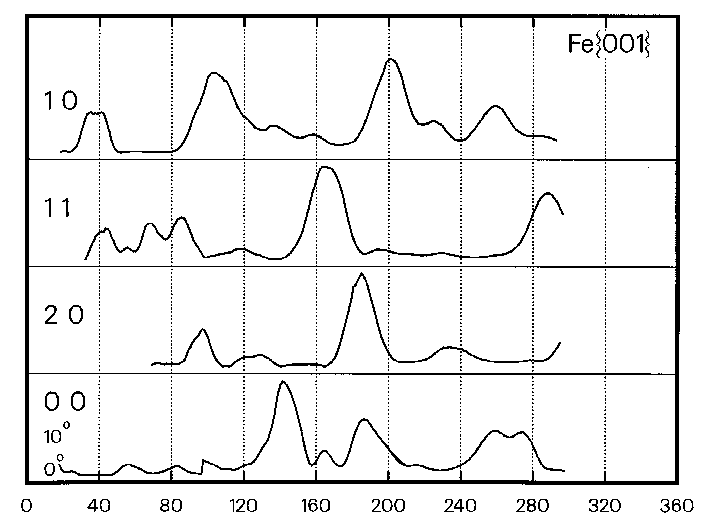
\includegraphics[width=\textwidth]{Plots/fe.png}
    \caption{}
  \end{subfigure}
  \begin{subfigure}{0.47\textwidth}
    \includegraphics[width=\textwidth]{Plots/IV-FeO_Layout.pdf}
    \caption{}
  \end{subfigure}
  \begin{subfigure}{0.47\textwidth}
    \vspace{-0.2cm}
    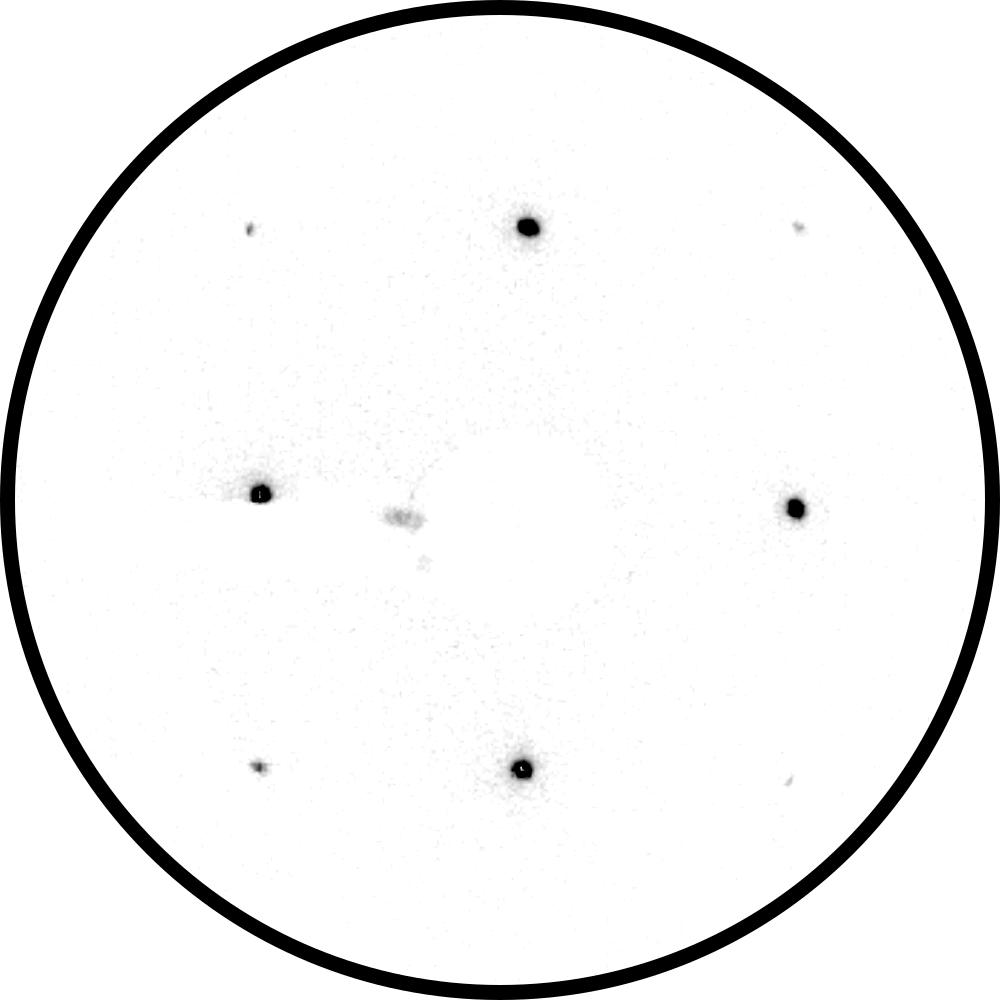
\includegraphics[width=\textwidth]{Plots/feO.png}
    \caption{}
  \end{subfigure}
  \begin{subfigure}{0.47\textwidth}
%    \vspace{-0.2cm}
    \includegraphics[width=\textwidth]{Plots/IV-MgO_Layout.pdf}
    \caption{}
  \end{subfigure}
  \begin{subfigure}{0.47\textwidth}
    \vspace{0.6cm}
    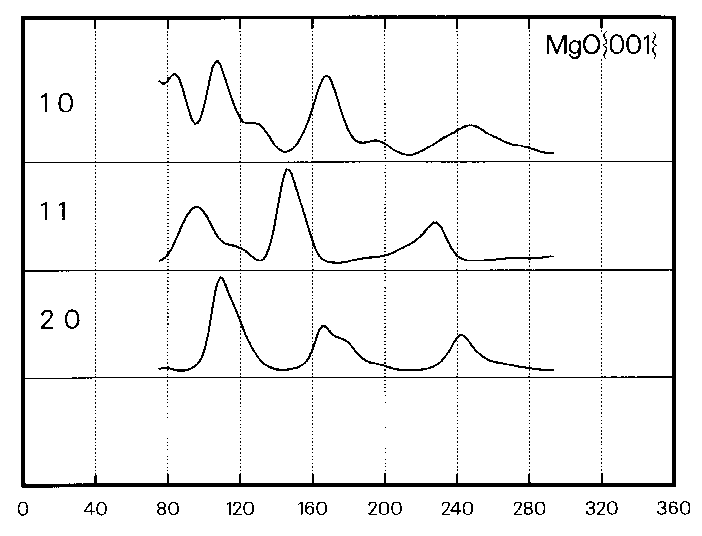
\includegraphics[width=\textwidth]{Plots/mgo.png}
    \caption{}
  \end{subfigure}
  \caption{Aufgenommene IV-Kurven links (a) von sauberem Fe(100), (c) sauberem Fe(100)-p(1\,x\,1)O und (e) MgO. 
          Der (00)-Reflex vom reinen Eisen wurde unter einem $15\,\si{\degree}$ Winkel aufgenommen, der vom passivierten Eisen bei $10\,\si{\degree}$.
          Durch einen Savitzky-Golay Filter 2. Ordnung mit 21 Punkten wurden die
          IV-Kurven geglättet.
          Rechts zum Vergleich Literaturdaten aus dem IV Data Repository \cite{IV}, welche den Daten aus \cite{PhysRevB.16.5271,Legg_1977,JONA1987667,URANO1983109} entsprechen.}%
  \label{fig:IV1}
\end{figure}


Für das reine Eisen, das mit Sauerstoff passivierte Eisen und einen dicken MgO-Film (mehr als 10\,ML)
wurden IV-Kurven aufgenommen. In Abbildung \ref{fig:IV1} ist ein Vergleich der gemessenen Kurven (links) für die 
drei Systeme mit der Literatur (rechts) gezeigt.
Bei dem (10)- und dem (11)-Reflex des passivierten Eisens sind Abweichungen bei den Peakhöhen zu erkennen.
Abgesehen davon liegt eine gute Übereinstimmung der restlichen Reflexe vor.
Die abweichenden Ergebnisse für das passivierte Eisen konnten mehrfach reproduziert werden.


Durch das sukzessive Wachstum ist es möglich, einen zeitlichen Verlauf der IV-Kurven aufzunehmen und Referenzdaten
für eine unterschiedliche Anzahl weniger Monolagen zu erhalten. In Abbildung \ref{fig:IV2} ist eine Zusammenstellung 
dieser IV-Kurven für den (10)-, den (11)- und den (20)-Reflex auf Fe(100) (links) und Fe(100)-p(1\,x\,1)O (rechts) zu sehen.


Die Markierungen zeigen Charakteristika verschiedener Schichtdicken.
Beim MgO-Wachstum auf reinem Eisen ist beim (10)-Reflex in Abbildung \ref{fig:IV2}(a) ein Peak 
bei $240$\,eV bei 1\,ML zu sehen, der bei den anderen vermessenen Schichtdicken nicht auftritt.\newline
Der (11)-Reflex in Abbildung \ref{fig:IV2}(c) zeigt einen Rückgang des $170$\,eV-Peaks vom sauberen Eisen Fe(100), welcher bei 1\,ML kleiner und ab $1,6$\,ML gar nicht mehr sichtbar ist.
Der $140$\,eV-Peak vom MgO-Verlauf ist bereits deutlich ab $1,6$\,ML sichtbar und bleibt bei höheren Schichtdicken konstant.\newline
Ebenso ist der $165$\,eV-Peak des (20)-Reflexes in Abbildung \ref{fig:IV2}(e) von MgO bereits ab $1,6$\,ML zu beobachten, wobei dieser 
bei $1,6$\,ML und $3,5$\,ML noch vom $190$\,eV-Peak überlagert wird. Letzterer nimmt mit zunehmender Schichtdicke an Intensität ab.

Beim MgO-Wachstum auf passiviertem Eisen zeigt der (10)-Reflex in Abbildung \ref{fig:IV2}(b) bereits ab einer Schichtdicke von 1,1\,ML den 
$165$\,eV-Peak von MgO.\newline 
Gleich verhält es sich mit dem $140$\,eV-Peak beim (11)-Reflex in Abbildung \ref{fig:IV2}(d).
Im Vergleich zum Wachstum auf reinem Eisen (siehe Abbildung \ref{fig:IV2}(c)) ist auffällig, dass dieser dort bei einer Schichtdicke von 1\,ML 
noch nicht sichtbar ist.\newline
Ähnlich wie beim (20)-Reflex des Wachstums auf reinem Eisen ist beim (20)-Reflex auf passiviertem Eisen in Abbildung \ref{fig:IV2}(f)
eine Überlagerung zweier Peaks zu sehen. Der $165$\,eV-Peak von MgO überlagert sich ab einer Schichtdicke von 1,1\,ML
mit dem $190$\,eV-Peak, wobei letzterer auch wieder mit steigender Schichtdicke abnimmt.
Wie beim $140$\,eV-Peak beim (11)-Reflex, ist der $190$\,eV-Peak hier beim Wachstum auf reinem Eisen (siehe Abbildung \ref{fig:IV2}(e)) bei einer Schichtdicke von
1\,ML noch nicht sichtbar.

Die aufgeführten Merkmale der IV-Kurven können genutzt werden, um verschiedene Schichtdicken der 
Systeme Fe(100)/MgO und Fe(100)-p(1\,x\,1)O/MgO zu identifizieren.


\begin{figure}[H]
   \centering
   \subfloat[][]{\includegraphics[width=0.47\linewidth]{Plots/IV-10_Layout.pdf}}%
   \qquad
   \subfloat[][]{\includegraphics[width=0.47\linewidth]{Plots/IV-10_FeO-Layout.pdf}}
   \qquad
   \subfloat[][]{\includegraphics[width=0.47\linewidth]{Plots/IV-11_Layout.pdf}}
   \qquad
   \subfloat[][]{\includegraphics[width=0.47\linewidth]{Plots/IV-11_FeO-Layout.pdf}}
   \qquad
   \subfloat[][]{\includegraphics[width=0.47\linewidth]{Plots/IV-20_Layout.pdf}}%
   \qquad
   \subfloat[][]{\includegraphics[width=0.47\linewidth]{Plots/IV-20_FeO-Layout.pdf}}
   \caption{IV-Kurven aufgenommen bei unterschiedlicher Schichtdicke von MgO auf Fe(100) (links) und MgO auf Fe(100)-p(1\,x\,1)O (rechts).
            (a) und (b) zeigen jeweils den (10)-Reflex, (c) und (d) den (11)-Reflex und (e) und (f) den (20)-Reflex.
            Durch einen Savitzky-Golay Filter 2. Ordnung mit 21 Punkten wurden die
          IV-Kurven geglättet.}%
   \label{fig:IV2}
\end{figure}
